\documentclass[xelatex,aspectratio=168]{beamer}

\hfuzz=10pt
\vfuzz=10pt

% Theme
\usetheme{htw}
\setbeamertemplate{navigation symbols}{}
\setbeamertemplate{theorems}[numbered]
\setbeamercovered{transparent}

%\logo{
\includegraphics[height=0.5cm]{HTWD_color.png}}

% Packages
\usepackage{polyglossia}
\setmainlanguage{german}
\setotherlanguage{english}

\usepackage[bigfiles]{pdfbase}
\ExplSyntaxOn
\NewDocumentCommand\embedvideo{smm}{
\group_begin:
\leavevmode
\tl_if_exist:cTF{file_\file_mdfive_hash:n{#3}}{
  \tl_set_eq:Nc\video{file_\file_mdfive_hash:n{#3}}
}{
  \IfFileExists{#3}{}{\GenericError{}{File~`#3'~not~found}{}{}}
  \pbs_pdfobj:nnn{}{fstream}{{}{#3}}
  \pbs_pdfobj:nnn{}{dict}{
    /Type/Filespec/F~(#3)/UF~(#3)
    /EF~<</F~\pbs_pdflastobj:>>
  }
  \tl_set:Nx\video{\pbs_pdflastobj:}
  \tl_gset_eq:cN{file_\file_mdfive_hash:n{#3}}\video
}
%
\pbs_pdfobj:nnn{}{dict}{
  /Type/RichMediaInstance/Subtype/Video
  /Asset~\video
  /Params~<</FlashVars (
  source=#3&
  skin=SkinOverAllNoFullNoCaption.swf&
  skinAutoHide=true&
  skinBackgroundColor=0x5F5F5F&
  skinBackgroundAlpha=0.75
  )>>
}
%
\pbs_pdfobj:nnn{}{dict}{
/Type/RichMediaConfiguration/Subtype/Video
/Instances~[\pbs_pdflastobj:]
}
%
\pbs_pdfobj:nnn{}{dict}{
/Type/RichMediaContent
/Assets~<<
/Names~[(#3)~\video]
>>
/Configurations~[\pbs_pdflastobj:]
}
\tl_set:Nx\rmcontent{\pbs_pdflastobj:}
%
\pbs_pdfobj:nnn{}{dict}{
  /Activation~<<
  /Condition/\IfBooleanTF{#1}{PV}{XA}
  /Presentation~<</Style/Embedded>>
  >>
  /Deactivation~<</Condition/PI>>
}
%
\hbox_set:Nn\l_tmpa_box{#2}
\tl_set:Nx\l_box_wd_tl{\dim_use:N\box_wd:N\l_tmpa_box}
\tl_set:Nx\l_box_ht_tl{\dim_use:N\box_ht:N\l_tmpa_box}
\tl_set:Nx\l_box_dp_tl{\dim_use:N\box_dp:N\l_tmpa_box}
\pbs_pdfxform:nnnnn{1}{1}{}{}{\l_tmpa_box}
%
\pbs_pdfannot:nnnn{\l_box_wd_tl}{\l_box_ht_tl}{\l_box_dp_tl}{
  /Subtype/RichMedia
  /BS~<</W~0/S/S>>
  /Contents~(embedded~video~file:#3)
  /NM~(rma:#3)
  /AP~<</N~\pbs_pdflastxform:>>
  /RichMediaSettings~\pbs_pdflastobj:
  /RichMediaContent~\rmcontent
}
\phantom{#2}
\group_end:
}
\ExplSyntaxOff


\usepackage{graphicx}
\usepackage[export]{adjustbox}
\usepackage{animate}
%\usepackage[dvipdfmx]{movie15_dvipdfmx}
\usepackage{media9}
\usepackage{tabularx}
\usepackage{colortbl}
\usepackage{booktabs}
\usepackage{makecell}
\usepackage{ltablex}
\usepackage{array}
\usepackage{multirow}
\usepackage{amsmath}
\usepackage{amsthm}
%\renewcommand{\arraystretch}{1.5}
\newcolumntype{L}[1]{>{\raggedright\let\newline\\\arraybackslash\hspace{0pt}}p{#1}}
\newcolumntype{C}[1]{>{\centering\let\newline\\\arraybackslash\hspace{0pt}}p{#1}}
\newcolumntype{R}[1]{>{\raggedleft\let\newline\\\arraybackslash\hspace{0pt}}p{#1}}
%\renewcommand\thesatz{\arabic{section}.\arabic{theorem}}
\makeatletter
\@addtoreset{theorem}{lecture}
\makeatother

\newtheorem{satz}{Satz}[section]
\newtheorem{lem}{Lemma}[section]
\newtheorem{beh}{Behauptung}[section]
\newtheorem{define}{Definition}[section]
\numberwithin{equation}{section}
\usepackage{ragged2e}
\usepackage{etoolbox}

\usepackage{color}
\usepackage{colortbl}
\definecolor{hellgrau}{rgb}{0.85,0.85,0.85}
\definecolor{hellrot}{rgb}{1,0.7,0.7}

\usepackage{tikz}
\usetikzlibrary{shapes,arrows.meta,calc,arrows,positioning,patterns,tikzmark}
%\usepackage{tikz-uml}
\usepackage{pgfplots}  % for elliptic curves (part 8)
\pgfplotsset{compat=1.18}
\usepackage{pgffor}
\usepackage{pgfmath-xfp}
\tikzset{>=latex}
\tikzset{
  invisible/.style={opacity=0},
  visible on/.style={alt={#1{}{invisible}}},
  alt/.code args={<#1>#2#3}{%
      \alt<#1>{\pgfkeysalso{#2}}{\pgfkeysalso{#3}} % \pgfkeysalso doesn't change the path
    },
}

\usepackage{paralist}

\usepackage{url}
\def\UrlBreaks{\do\/\do-}
\PassOptionsToPackage{hyphens}{url}\usepackage{hyperref}

\usepackage[normalem]{ulem} % gestrichelte Unterstreichung (\dashuline{})
\usepackage{cancel}

\makeatletter
\renewcommand{\itemize}[1][]{%
  \beamer@ifempty{#1}{}{\def\beamer@defaultospec{#1}}%
  \ifnum \@itemdepth >2\relax\@toodeep\else
    \advance\@itemdepth\@ne
    \beamer@computepref\@itemdepth% sets \beameritemnestingprefix
    \usebeamerfont{itemize/enumerate \beameritemnestingprefix body}%
    \usebeamercolor[fg]{itemize/enumerate \beameritemnestingprefix body}%
    \usebeamertemplate{itemize/enumerate \beameritemnestingprefix body begin}%
    \list
    {\usebeamertemplate{itemize \beameritemnestingprefix item}}
    {\def\makelabel##1{%
        {%
            \hss\llap{{%
                  \usebeamerfont*{itemize \beameritemnestingprefix item}%
                  \usebeamercolor[fg]{itemize \beameritemnestingprefix item}##1}}%
          }%
      }%
    }
  \fi%
  \beamer@cramped%
  \justifying% NEW
  %\raggedright% ORIGINAL
  \beamer@firstlineitemizeunskip%
}
\makeatother

\apptocmd{\frame}{}{\justifying}{}

\renewcommand\theadfont{\bfseries\sffamily}
\usepackage{ragged2e}
\usepackage{newpxtext}

\setsansfont{texgyreheros}[
  Scale=MatchLowercase,
  UprightFont=*-regular,
  BoldFont=*-bold,
  ItalicFont=*-italic,
  BoldItalicFont=*-bolditalic,
]

% Title
\usepackage[usetransparent=false]{svg}
% Import references
\usepackage[backend=biber,style=numeric,sorting=none]{biblatex}
\addbibresource{references.bib}

%\AtBeginSection[]{
%  \begin{frame}
%    \vfill
%    \centering
%    \begin{beamercolorbox}[sep=8pt,center,shadow=true,rounded=true]{title}
%      \usebeamerfont{title}\thesection.~\secname\par%
%    \end{beamercolorbox}
%    \vfill
%  \end{frame}
%}

\makeatletter
\newenvironment{noheadline}{
  \setbeamertemplate{headline}{}
  \addtobeamertemplate{frametitle}{\vspace*{-0.9\baselineskip}}{}
}{}
\makeatother


\usepackage{xcolor}
\usepackage{algorithm}
\usepackage[linesnumbered,ruled,lined,commentsnumbered,algo2e,ngerman,ngermankw]{algorithm2e}
\usepackage{algorithmic}
\usepackage{caption}
\usepackage[newfloat]{minted}
\captionsetup[listing]{position=top}
\definecolor{mintedbg}{HTML}{282828}
\setminted{
  breaklines=true,
  bgcolor=mintedbg,
  style=monokai,
  formatcom=\color{white}
}
\usepackage{etoolbox}
\makeatletter
% replace \medskip before and after the box with nothing, i.e., remove it
\patchcmd{\minted@colorbg}{\medskip}{}{}{}
\patchcmd{\endminted@colorbg}{\medskip}{}{}{}
\makeatother

\renewcommand{\theFancyVerbLine}{\textcolor{black}{\arabic{FancyVerbLine}}}

\usepackage{pifont}
\newcommand{\cmark}{\ding{51}}%
\newcommand{\xmark}{\ding{55}}%

\newenvironment{changemargin}[2]{%
  \begin{list}{}{%
      \setlength{\topsep}{0pt}%
      \setlength{\leftmargin}{#1}%
      \setlength{\rightmargin}{#2}%
      \setlength{\listparindent}{\parindent}%
      \setlength{\itemindent}{\parindent}%
      \setlength{\parsep}{\parskip}%
    }%
    \item[]}{\end{list}}


\usepackage{csquotes}

% Title
\title{Organisatorisches}
\author{Prof. Dr. Lukas Iffländer}
\institute{HTW Dresden}
\date{}
\usepackage{svg}

% Begin document
\begin{document}

% Title slide
\begin{frame}
  \titlepage
\end{frame}

\section{Vorstellung}

\begin{frame}{Euer Prof}
  \begin{columns}
    \begin{column}{.4\textwidth}
      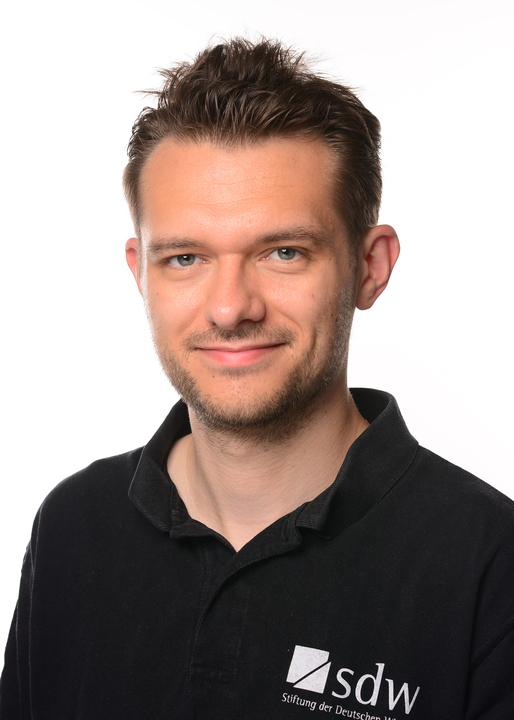
\includegraphics[height=.8\textheight]{img/portrait.jpg}
    \end{column}
    \begin{column}{.5\textwidth}
      \begin{itemize}
        \item Prof. Dr. Lukas Iffländer
        \item Raum: U 452
        \item E-Mail: \url{lukas.ifflaender@htw-dresden.de}
        \item Telefon: +49 351 462 3516
      \end{itemize}
    \end{column}
  \end{columns}
\end{frame}

\begin{frame}{Lebenslauf}{Ausbildung}
  \begin{description}
    \item<1->[1990] Geboren in Neustadt a.d. Waldnaab \vspace{15pt}

    \item<2->[1996--2009] Grundschule und Abitur in Weiden in der Oberpfalz
    \item<2->[2009--2012] Bachelor Luft- und Raumfahrtinformatik in Würzburg
    \item<2->[2012--2016] Master Informatik in Würzburg
    \item<2->[2016--2021] Promotion Informatik mit Schwerpunkt Cybersecurity in Würzburg
  \end{description}
\end{frame}

\begin{frame}{Lebenslauf}{Berufserfahrung}
  \begin{description}
    \item[2009] Praktikum bei Siemens Industrial Solutions in Erlangen
    \item[2010--2012] Werkstudent bei Siemens Industrial Solutions in Erlangen
    \item[2012--2014] Werkstudent bei Siemens Infrastructure \& Cities in Erlangen
    \item[2010--2015] Wissenschaftliche Hilfskraft bei Uni und FH in Würzburg
    \item[2015--2018] Wissenschaftlicher Mitarbeiter bei Uni Würzburg
    \item[2018--2020] Forschungsgruppenleiter bei Uni Würzburg
    \item[2020--2024] Wissenschaftlicher Referent am Deutschen Zentrum für Schienenverkehrsforschung
    \item[seit 2024] Professor für Informationssicherheit an der HTW-Dresden
  \end{description}
\end{frame}

\begin{frame}{Lebenslauf}{Ehrenamt}
  \begin{itemize}
    \item Fahrgastverband PRO BAHN
          \begin{description}
            \item[2011--2012] Pressesprecher Mittel- und Oberfranken
            \item[2012--2021] Stellvertretender Landesvorsitzender Bayern
            \item[seit 2016] Stellvertretender Bundesvorsitzender
            \item[seit 2021] Landesvorsitzender Bayern
          \end{description}
    \item Uni Würzburg
          \begin{description}
            \item[2020-2023] Forschungsgruppenleiter
          \end{description}
  \end{itemize}
\end{frame}

\section{Organisatorisches}

% Content slides
\begin{frame}
  \frametitle{Informationen}
  Wichtige Informationen zur Vorlesung findet ihr im OPAL-Kurs.

  \begin{block}{OPAL-Kurs}
    \begin{center}
      \url{https://t1p.de/htwd-maschb-info}
    \end{center}
  \end{block}
\end{frame}

\begin{frame}
  \frametitle{Termine}
  \begin{itemize}
    \item Vorlesung: Mittwoch, 15:30 - 17:00 Uhr Raum Z107
    \item Tutorium: Freitag (ungerade Wochen), 9:45 - 11:15 Uhr Raum S239
    \item Labor: Dienstag 08:00-09:30 Raum U 522
    \item Labor: Dienstag 09:45-11:15 Raum U 522
    \item Labor: Freitag 11:30-13:00 Raum U 523
    \item Labor: Freitag 13:45-15:15 Raum U 523
  \end{itemize}

  \begin{block}{Labor}
    Im Labor werden Übungsblätter bearbeitet und Fragen beantwortet.
  \end{block}

  \begin{block}{Tutorium}
    Das Tutorium kann für freies Lernen genutzt werden (Übungsblätter, Fragen stellen, Hobbyprojekte). Im Tutorium sind keine Rechner vorhanden, bitte eigenen Laptop mitbringen.
  \end{block}
\end{frame}

\begin{frame}{Übungsanmeldung}
  Euer Stundenplan ist nicht \enquote{stabil}, da es Kolissionen mit anderen Veranstaltungen/Laboren gibt. Bitte meldet euch daher jede Woche über OPAL zu den Laborgruppen an.
  \begin{block}{Anmeldung}
    \begin{itemize}
      \item Anmeldung zu den Laborgruppen über OPAL verpflichtend.
      \item Plätze sind beschränkt (max. 24 Studierende pro Gruppe).
      \item Bitte seid ehrlich und fair und meldet euch wieder ab, falls ihr doch nicht teilnehmen könnt.
      \item Sind am Vorabend um 22 Uhr keine Anmeldungen vorhanden, fällt die Laborgruppe aus.
    \end{itemize}
  \end{block}
\end{frame}

\begin{frame}{Arbeitsaufwand}
  \begin{exampleblock}{Umrechnug}
    1 ECTS entspricht ca. 30 Stunden
  \end{exampleblock}
  \begin{block}{Arbeitsaufwand}
    \begin{itemize}
      \item 5 ECTS entsprechen ca. 150 Stunden
      \item 30 Stunden Vorlesung
      \item 15 Stunden Tutorium
      \item 30 Stunden Labor
      \item 75 Stunden Selbststudium
    \end{itemize}
  \end{block}
  \begin{alertblock}{Programmieren muss man üben}
    \begin{itemize}
      \item Programmierung ist ein Handwerk
      \item Als solches muss es regelmäßig geübt werden, bis es ins Muskelgedächtnis übergeht
      \item Es ist wichtig, Fehler zu machen und daraus zu wachsen
    \end{itemize}
  \end{alertblock}

\end{frame}

\begin{frame}{Team}
  \begin{columns}
    \begin{column}{.3\textwidth}
      \begin{block}{Prof. Dr. Lukas Iffländer}
        \centering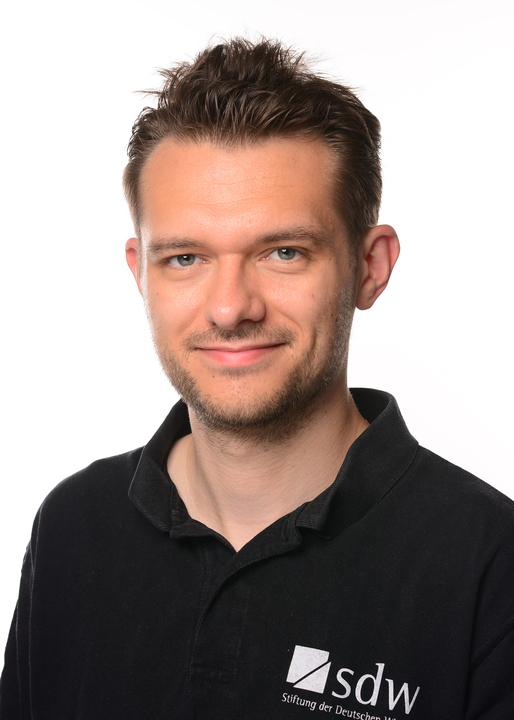
\includegraphics[height=.55\textheight]{img/portrait.jpg}
      \end{block}
    \end{column}
    \begin{column}{.35\textwidth}
      \begin{block}{Prof. Dr. Peter Sobe}
        \centering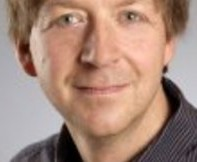
\includegraphics[height=.55\textheight]{img/sobe.jpg}
      \end{block}
    \end{column}
    \begin{column}{.30\textwidth}
      \begin{block}{Alexander Wülfing}
        \centering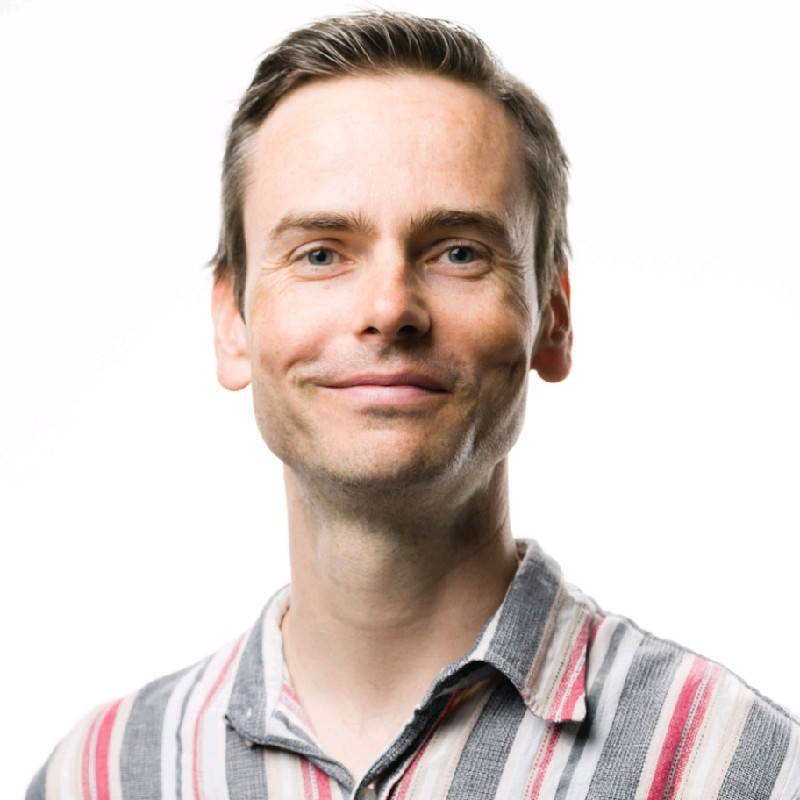
\includegraphics[height=.55\textheight]{img/wuelfing.jpg}
      \end{block}
    \end{column}
  \end{columns}
\end{frame}

\begin{frame}{Kauft euch einen Laptop}
  \begin{itemize}
    \item Ich empfehle dringend, dass ihr euch einen Laptop kauft, falls noch nicht passiert.
    \item Viele Übungen gehen nur mit einem ``echten'' Betriebssystem (nicht Android oder iOS). Mac oft schwierig.
          \begin{columns}[T]
            \begin{column}{.5\textwidth}
              \begin{block}{Empfehlung Low Budget}
                \begin{itemize}
                  \item Gebrauchtes ThinkPad (T, X, W, P Serie)
                  \item mindestens Quad-Core CPU
                  \item mindestens 16 GB RAM
                  \item Beispiele: % Rechtschreibung korrigiert
                        \begin{itemize}
                          \item X390 (i5, 16 GB RAM) für ca. 300 EUR
                          \item T14 Gen 1 (Ryzen 7, 32 GB RAM) für ca. 500 EUR
                        \end{itemize}
                  \item Gute Erfahrungen mit \url{https://www.luxnote-hannover.de/}
                \end{itemize}
              \end{block}
            \end{column}
            \begin{column}{.5\textwidth}
              \begin{block}{Empfehlung High Budget}
                \begin{itemize}
                  \item Neues Thinkpad (T, X, W, P Serie)
                  \item mindestens Octa-Core CPU
                  \item mindestens 32 GB RAM
                  \item Beispiele: % Rechtschreibung korrigiert
                        \begin{itemize}
                          \item Ultra-leicht: ThinkPad X1 Carbon % Bindestrich hinzugefügt
                          \item Leichtes Powerhorse: ThinkPad T14s (AMD mit Ryzen 7) % Zusammenschreibung korrigiert
                        \end{itemize}
                  \item Zahlreiche Anbieter im Lenovo Campus Programm (z.B. \url{https://www.campuspoint.de/})
                \end{itemize}
              \end{block}
            \end{column}
          \end{columns}
  \end{itemize}
  Beratung gerne wenn Zeit ist in den Übungen oder im Tutorium.
\end{frame}

\begin{frame}{Übungen zuhause machen}
  Wer die Aufgaben zum Selbststudium nicht in den Laborräumen machen möchte, kann diese auch zuhause bearbeiten.
  \begin{block}{Voraussetzungen}
    \begin{itemize}
      \item Aktuelles Python
      \item Eine IDE
            \begin{itemize}
              \item Spyder (sehr einfach, ideal zum lernen)
              \item Visual Studio Code (mächtiger und komplexer, aber auch mehr Funktionen)
              \item PyCharm (sehr mächtig, aber auch sehr komplex)
            \end{itemize}
      \item Empfehlung: Lasst am Anfang KIs wie Github Copilot oder Kite aus, um das Programmieren zu lernen. Dagegen darf man ChatGPT gerne mal fragen, warum der Code nicht funktioniert.
    \end{itemize}
  \end{block}
\end{frame}

\begin{frame}{Literaturempfehlungen}
  \begin{itemize}
    \item \fullcite{Schneider_2012_TaschenbuchDerInformatik}
    \item \fullcite{Kofler_2020_Python}
    \item \fullcite{Klein_2023_NumerischesPython}
  \end{itemize}
  Alle Bücher sind in der Bibliothek verfügbar.
\end{frame}

\begin{frame}{Prüfung}
  \begin{block}{Schriftliche Prüfungsleistung}
    \begin{itemize}
      \item Schriftliche Prüfung (elektronisch in den Laboren)
      \item Dauer 90 Minuten
      \item Hilfsmittel: Open Book (Skript, eigene Notizen, eigene Übungsblätter)
    \end{itemize}
  \end{block}
  \begin{block}{Prüfungsvorleistung}
    \begin{itemize}
      \item Aufgabe selbstständig in Python zu bearbeiten, dokumentieren und abzugeben
            \begin{itemize}
              \item Ausgabe: Mai 2025
              \item Abgabe: Mitte Juni 2025
            \end{itemize}
      \item Nur nach Bestehen der Prüfungsvorleistung ist die Teilnahme an der schriftlichen Prüfung (elektronisch in den Laboren) möglich
    \end{itemize}
  \end{block}
\end{frame}

% Conclusion slide
\begin{frame}
  \frametitle{Eine Vorlesung ist ein atmendes System}
  \begin{alertblock}{Bitte um ehrliches Feedback}
    \begin{itemize}
      \item Bitte gebt mir ehrliches Feedback, was gut und was schlecht läuft.
      \item Ihr habt die Chance, Dinge mitzugestalten, sodass sie für nachfolgende Studis noch besser sind. % Zusammenschreibung korrigiert
      \item Wenn etwas schief geht, wird das nicht zu euren Ungunsten laufen. % Rechtschreibung korrigiert
    \end{itemize}
  \end{alertblock}
\end{frame}

% End document
\end{document}
